\documentclass[11pt,letterpaper]{article}

% ============================================================================
% PACKAGES
% ============================================================================
\usepackage[margin=1in]{geometry}
\usepackage{schemabloc}          % Control system block diagrams
\usepackage{tikz}                % Required by schemabloc
\usepackage{amsmath,amssymb}     % Math equations
\usepackage{tcolorbox}           % Colored boxes for callouts
\usepackage{booktabs}            % Nice tables
\usepackage{graphicx}            % Include figures
\usepackage{hyperref}            % Clickable links in PDF
\usepackage{xcolor}              % Colors
\usepackage{enumitem}            % Better lists
\usepackage{fancyhdr}            % Headers/footers
\usepackage{titlesec}            % Section formatting
\usepackage{siunitx}             % SI units
\usepackage{float}               % Better float placement

% ============================================================================
% DOCUMENT SETTINGS
% ============================================================================
\hypersetup{
    colorlinks=true,
    linkcolor=blue!60!black,
    urlcolor=blue!60!black
}

% Header/Footer
\pagestyle{fancy}
\fancyhf{}
\fancyhead[L]{\small ESET 462 Control Systems Primer}
\fancyhead[R]{\small STAR Autonomous Robot}
\fancyfoot[C]{\thepage}

% Section formatting
\titleformat{\section}{\Large\bfseries\color{blue!60!black}}{\thesection}{1em}{}
\titleformat{\subsection}{\large\bfseries}{\thesubsection}{1em}{}

% Custom colored boxes
\newtcolorbox{plainenglish}{
    colback=green!5!white,
    colframe=green!50!black,
    title={\textbf{In Plain English}},
    fonttitle=\bfseries
}

\newtcolorbox{whymatters}{
    colback=blue!5!white,
    colframe=blue!50!black,
    title={\textbf{Why This Matters}},
    fonttitle=\bfseries
}

\newtcolorbox{keypoint}{
    colback=yellow!10!white,
    colframe=orange!70!black,
    title={\textbf{Key Point}},
    fonttitle=\bfseries
}

\newtcolorbox{ournumbers}{
    colback=gray!5!white,
    colframe=gray!50!black,
    title={\textbf{STAR Project Values}},
    fonttitle=\bfseries
}

\newtcolorbox{safetynote}{
    colback=red!5!white,
    colframe=red!50!black,
    title={\textbf{Safety Critical}},
    fonttitle=\bfseries
}

% ============================================================================
% DOCUMENT START
% ============================================================================
\begin{document}

% ----------------------------------------------------------------------------
% TITLE PAGE
% ----------------------------------------------------------------------------
\begin{titlepage}
    \centering
    \vspace*{2cm}

    {\Huge\bfseries Control Systems Primer\\[0.5cm]}
    {\Large A Guide to Understanding the STAR Robot Control Architecture\\[2cm]}

    {\large\textbf{STAR: Autonomous Mapping Robot}\\[0.5cm]}
    {\large ESET 462 -- Control Systems\\[0.3cm]}
    {\large Texas A\&M University\\[0.3cm]}
    {\large Fall 2025\\[2cm]}

    \vfill

    {\large\textbf{Team Members:}\\[0.3cm]}
    Elizabeth Ajose \quad Abhiraj Lakkamraju \quad Jacob Lopez\\
    Jackson Lopez \quad Cesar Magana \quad Ryan Ingram \quad Nafi Islam

    \vfill

    {\small\textit{Read this document to understand the control systems architecture of the STAR robot!}}
\end{titlepage}

\tableofcontents
\newpage

% ============================================================================
% CHAPTER 1: SYSTEM OVERVIEW
% ============================================================================
\section{System Overview}

\subsection{What is the STAR Robot?}

The STAR (Simultaneous Localization and Mapping) robot is an autonomous mobile platform designed to map indoor environments. It uses a sophisticated control system architecture with two main processing layers:

\begin{enumerate}
    \item \textbf{Navigation Layer (Raspberry Pi 5):} Runs ROS2 Nav2 with Hector-SLAM for mapping and path planning
    \item \textbf{Motor Control Layer (ESP32):} Executes cascaded PID control for precise motor control at 50Hz
\end{enumerate}

\begin{plainenglish}
Think of it like a self-driving car in miniature. The Raspberry Pi is the ``brain'' that decides where to go (using SLAM and path planning), while the ESP32 is the ``reflexes'' that make the wheels turn smoothly and safely.
\end{plainenglish}

\subsection{System Topology}

\begin{center}
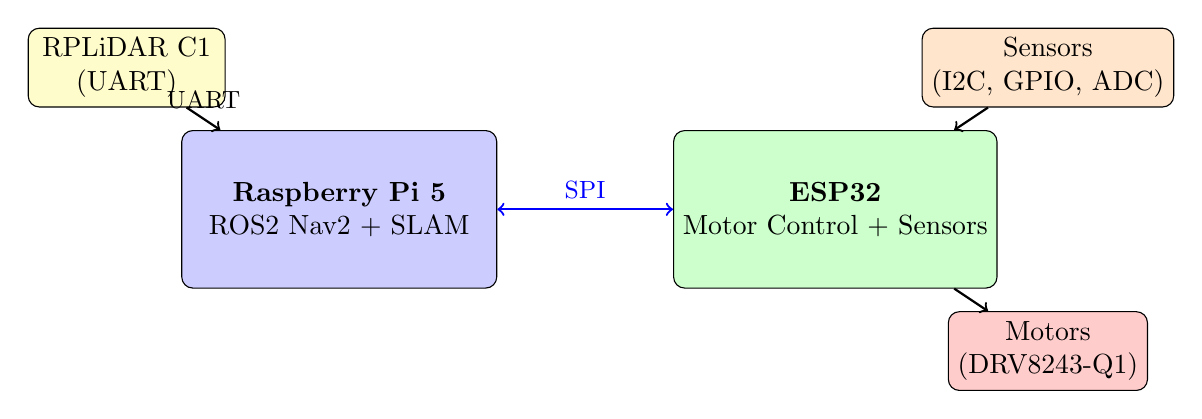
\begin{tikzpicture}[scale=0.9]
    % RPi5 block
    \node[draw, fill=blue!20, rounded corners, minimum width=4cm, minimum height=2cm, align=center] (rpi5) at (0,0) {
        \textbf{Raspberry Pi 5}\\
        ROS2 Nav2 + SLAM
    };

    % ESP32 block
    \node[draw, fill=green!20, rounded corners, minimum width=4cm, minimum height=2cm, align=center] (esp32) at (7,0) {
        \textbf{ESP32}\\
        Motor Control + Sensors
    };

    % LiDAR
    \node[draw, fill=yellow!20, rounded corners, minimum width=2.5cm, minimum height=1cm, align=center] (lidar) at (-3,2) {
        RPLiDAR C1\\
        (UART)
    };

    % Sensors
    \node[draw, fill=orange!20, rounded corners, minimum width=2.5cm, minimum height=1cm, align=center] (sensors) at (10,2) {
        Sensors\\
        (I2C, GPIO, ADC)
    };

    % Motors
    \node[draw, fill=red!20, rounded corners, minimum width=2.5cm, minimum height=1cm, align=center] (motors) at (10,-2) {
        Motors\\
        (DRV8243-Q1)
    };

    % Connections
    \draw[->, thick] (lidar) -- (rpi5) node[midway, above] {\small UART};
    \draw[<->, thick, blue] (rpi5) -- (esp32) node[midway, above] {\small SPI};
    \draw[->, thick] (sensors) -- (esp32);
    \draw[->, thick] (esp32) -- (motors);
\end{tikzpicture}
\end{center}

\subsection{Control System Hierarchy}

Our robot uses a \textbf{hierarchical control architecture}:

\begin{table}[H]
\centering
\begin{tabular}{@{}llll@{}}
\toprule
\textbf{Level} & \textbf{Processor} & \textbf{Function} & \textbf{Rate} \\
\midrule
Planning & RPi5 & Global path planning (A* algorithm) & 1 Hz \\
Navigation & RPi5 & Local planning (DWA) & 10 Hz \\
Velocity & ESP32 & Velocity setpoint tracking & 50 Hz \\
Current & ESP32 & Motor current regulation & 50 Hz \\
Safety & ESP32 & Supervisory override & 50 Hz \\
\bottomrule
\end{tabular}
\caption{Control hierarchy from high-level planning to low-level actuation}
\end{table}

\begin{whymatters}
This hierarchical approach separates concerns: the RPi5 handles computationally expensive SLAM and planning, while the ESP32 handles time-critical motor control. This ensures smooth motion even when the Pi is busy processing sensor data.
\end{whymatters}

% ============================================================================
% CHAPTER 2: CASCADED PID CONTROL
% ============================================================================
\newpage
\section{Cascaded PID Control Architecture}

\subsection{Why Cascaded Control?}

A single PID controller works well for simple systems, but our robot needs precise control of both position and velocity while protecting the motors from overcurrent. We achieve this with \textbf{cascaded PID loops}.

\begin{plainenglish}
Imagine a thermostat that not only controls room temperature but also monitors how fast the furnace is heating and how much fuel it's using. Each ``loop'' handles one aspect, and they work together like nested layers of control.
\end{plainenglish}

\subsection{The Three Control Loops}

\begin{center}
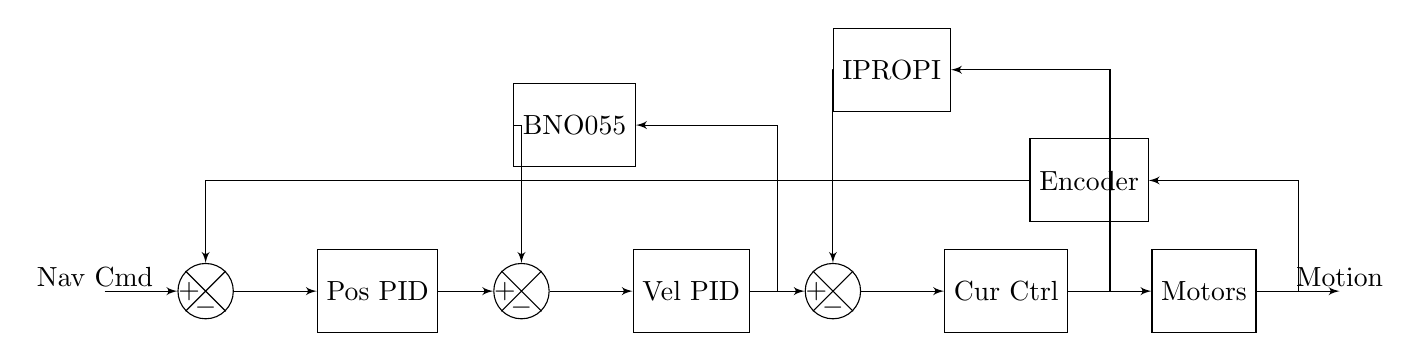
\begin{tikzpicture}
    % Navigation setpoint from ROS2
    \sbEntree{E}
    \sbComp{possum}{E}
    \sbBloc[3]{pospid}{Pos PID}{possum}
    \sbComp[3]{velsum}{pospid}
    \sbBloc[3]{velpid}{Vel PID}{velsum}
    \sbComp[3]{cursum}{velpid}
    \sbBloc[3]{curctrl}{Cur Ctrl}{cursum}
    \sbBloc[3]{motors}{Motors}{curctrl}
    \sbSortie[3]{S}{motors}

    % Main chain connections
    \sbRelier{E}{possum}
    \sbRelier{possum}{pospid}
    \sbRelier{pospid}{velsum}
    \sbRelier{velsum}{velpid}
    \sbRelier{velpid}{cursum}
    \sbRelier{cursum}{curctrl}
    \sbRelier{curctrl}{motors}
    \sbRelier{motors}{S}
    \sbNomLien[0.5]{E}{Nav Cmd}
    \sbNomLien[0.5]{S}{Motion}

    % Position feedback (encoder)
    \sbDecaleNoeudy[-4]{motors}{encfb}
    \sbBlocr{enc}{Encoder}{encfb}
    \sbRelieryx{motors-S}{enc}
    \sbRelierxy{enc}{possum}

    % Velocity feedback (BNO055)
    \sbDecaleNoeudy[-6]{velpid}{bnofb}
    \sbBlocr{bno}{BNO055}{bnofb}
    \sbRelieryx{velpid-cursum}{bno}
    \sbRelierxy{bno}{velsum}

    % Current feedback (IPROPI)
    \sbDecaleNoeudy[-8]{curctrl}{iprfb}
    \sbBlocr{ipr}{IPROPI}{iprfb}
    \sbRelieryx{curctrl-motors}{ipr}
    \sbRelierxy{ipr}{cursum}
\end{tikzpicture}
\end{center}

\subsubsection{Position Loop (Outer Loop)}
\begin{itemize}
    \item \textbf{Setpoint:} Desired position from ROS2 Nav2
    \item \textbf{Feedback:} Quadrature encoders on each motor
    \item \textbf{Output:} Velocity setpoint for the velocity loop
    \item \textbf{Purpose:} Ensure the robot reaches the commanded position
\end{itemize}

\subsubsection{Velocity Loop (Middle Loop)}
\begin{itemize}
    \item \textbf{Setpoint:} Velocity command from position loop
    \item \textbf{Feedback:} BNO055 IMU linear acceleration (integrated) + encoder derivative
    \item \textbf{Output:} Current setpoint for the current loop
    \item \textbf{Purpose:} Maintain smooth, consistent wheel speed
\end{itemize}

\subsubsection{Current Loop (Inner Loop)}
\begin{itemize}
    \item \textbf{Setpoint:} Current command from velocity loop
    \item \textbf{Feedback:} DRV8243-Q1 IPROPI analog current sense
    \item \textbf{Output:} PWM duty cycle to motor driver
    \item \textbf{Purpose:} Protect motors from overcurrent, ensure torque control
\end{itemize}

\begin{keypoint}
\textbf{Loop Bandwidth Rule:} Each inner loop must be 5-10x faster than its outer loop. Our current loop runs at the full 50Hz, velocity loop effectively at 50Hz with filtered feedback, and position loop commands come at 10Hz from Nav2.
\end{keypoint}

\subsection{Transfer Function Analysis}

Each loop can be modeled with its own transfer function:

\subsubsection{Motor Electrical Model}
The DC motor armature circuit is modeled as:
\begin{equation}
G_{motor}(s) = \frac{I(s)}{V(s)} = \frac{1}{Ls + R}
\end{equation}

Where:
\begin{itemize}
    \item $L$ = Motor inductance (\SI{0.5}{\milli\henry} typical)
    \item $R$ = Motor resistance (\SI{1.5}{\ohm} typical)
\end{itemize}

\subsubsection{Motor Mechanical Model}
The mechanical dynamics:
\begin{equation}
G_{mech}(s) = \frac{\omega(s)}{I(s)} = \frac{K_t}{Js + b}
\end{equation}

Where:
\begin{itemize}
    \item $K_t$ = Torque constant (\SI{0.01}{\newton\meter\per\ampere})
    \item $J$ = Rotor inertia (\SI{1e-5}{\kilogram\meter\squared})
    \item $b$ = Viscous friction (\SI{1e-4}{\newton\meter\second})
\end{itemize}

\begin{ournumbers}
\textbf{Estimated Plant Parameters:}
\begin{itemize}[noitemsep]
    \item Motor resistance: $R = \SI{1.5}{\ohm}$
    \item Motor inductance: $L = \SI{0.5}{\milli\henry}$
    \item Torque constant: $K_t = \SI{0.01}{\newton\meter\per\ampere}$
    \item Electrical time constant: $\tau_e = L/R = \SI{0.33}{\milli\second}$
    \item Mechanical time constant: $\tau_m = J/b = \SI{0.1}{\second}$
\end{itemize}
\end{ournumbers}

\subsection{PID Tuning Approach}

We use a \textbf{sequential tuning} approach:

\begin{enumerate}
    \item \textbf{Tune current loop first} (innermost, fastest)
    \begin{itemize}
        \item High bandwidth for fast current response
        \item Primarily P control with small I for offset correction
    \end{itemize}

    \item \textbf{Tune velocity loop second}
    \begin{itemize}
        \item Moderate bandwidth (5-10x slower than current loop)
        \item PI control for zero steady-state velocity error
    \end{itemize}

    \item \textbf{Tune position loop last} (outermost, slowest)
    \begin{itemize}
        \item Lowest bandwidth to prevent oscillation
        \item Often P-only or PI with very small integral gain
    \end{itemize}
\end{enumerate}

\begin{ournumbers}
\textbf{Initial PID Gains (to be tuned):}
\begin{itemize}[noitemsep]
    \item \textbf{Current Loop:} $K_p = 5.0$, $K_i = 100$, $K_d = 0$
    \item \textbf{Velocity Loop:} $K_p = 2.0$, $K_i = 0.5$, $K_d = 0.05$
    \item \textbf{Position Loop:} $K_p = 1.0$, $K_i = 0.1$, $K_d = 0$
\end{itemize}
\end{ournumbers}

% ============================================================================
% CHAPTER 3: SENSOR INTEGRATION
% ============================================================================
\newpage
\section{Sensor Integration}

\subsection{Sensor Overview}

The STAR robot uses multiple sensors for feedback and safety:

\begin{table}[H]
\centering
\begin{tabular}{@{}llll@{}}
\toprule
\textbf{Sensor} & \textbf{Interface} & \textbf{Purpose} & \textbf{Processor} \\
\midrule
RPLiDAR C1 & UART & SLAM mapping & RPi5 \\
BNO055 IMU & I2C & Orientation, velocity & ESP32 \\
DS18B20+ & OneWire & Temperature compensation & ESP32 \\
HC-SR04 & GPIO & Proximity safety & ESP32 \\
DRV8243 IPROPI & ADC & Current sensing & ESP32 \\
Quadrature Encoders & GPIO & Position feedback & ESP32 \\
BQ78350 Fuel Gauge & SMBus & Battery monitoring & ESP32 \\
\bottomrule
\end{tabular}
\caption{Sensor assignments and interfaces}
\end{table}

\subsection{BNO055 IMU Integration}

The BNO055 provides critical feedback for the velocity control loop:

\begin{center}
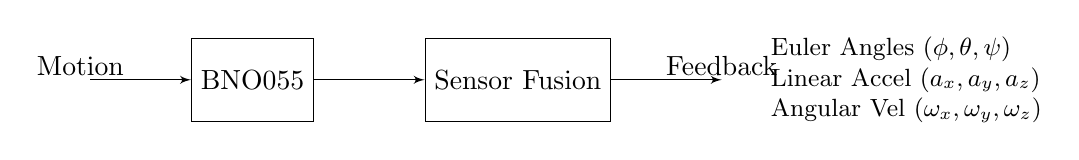
\begin{tikzpicture}
    \sbEntree{E}
    \sbBloc[4]{bno}{BNO055}{E}
    \sbBloc[4]{fuse}{Sensor Fusion}{bno}
    \sbSortie[4]{S}{fuse}

    \sbRelier{E}{bno}
    \sbRelier{bno}{fuse}
    \sbRelier{fuse}{S}

    \sbNomLien[0.5]{E}{Motion}
    \sbNomLien[0.5]{S}{Feedback}

    % Output branches
    \node[right=0.5cm of S, align=left, font=\small] {
        Euler Angles $(\phi, \theta, \psi)$\\
        Linear Accel $(a_x, a_y, a_z)$\\
        Angular Vel $(\omega_x, \omega_y, \omega_z)$
    };
\end{tikzpicture}
\end{center}

\textbf{BNO055 Outputs Used:}
\begin{itemize}
    \item \textbf{Orientation (Euler angles):} Heading feedback for heading PID
    \item \textbf{Linear acceleration:} Velocity estimation via integration
    \item \textbf{Gyroscope:} Angular velocity for turn rate feedback
\end{itemize}

\begin{keypoint}
The BNO055 has an onboard sensor fusion processor that combines accelerometer, gyroscope, and magnetometer data. This offloads computation from the ESP32 and provides drift-corrected orientation.
\end{keypoint}

\subsection{Temperature-Compensated Distance Measurement}

The HC-SR04 ultrasonic sensor's accuracy depends on the speed of sound, which varies with temperature. We use the DS18B20+ for compensation:

\begin{center}
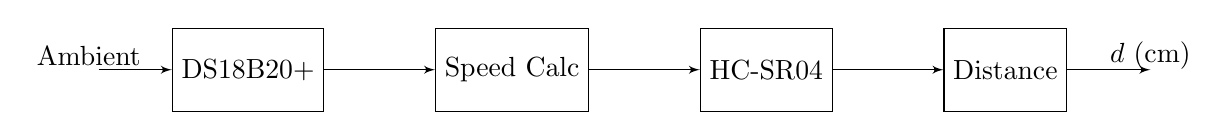
\begin{tikzpicture}
    \sbEntree{E}
    \sbBloc[3]{ds18}{DS18B20+}{E}
    \sbBloc[4]{calc}{Speed Calc}{ds18}
    \sbBloc[4]{hcsr}{HC-SR04}{calc}
    \sbBloc[4]{dist}{Distance}{hcsr}
    \sbSortie[3]{S}{dist}

    \sbRelier{E}{ds18}
    \sbRelier{ds18}{calc}
    \sbRelier{calc}{hcsr}
    \sbRelier{hcsr}{dist}
    \sbRelier{dist}{S}

    \sbNomLien[0.5]{E}{Ambient}
    \sbNomLien[0.5]{S}{$d$ (cm)}
\end{tikzpicture}
\end{center}

\textbf{Temperature Compensation Formula:}
\begin{equation}
v_{sound} = 331.3 + 0.606 \cdot T
\end{equation}

Where $T$ is temperature in Celsius and $v_{sound}$ is in m/s.

\textbf{Distance Calculation:}
\begin{equation}
d = \frac{v_{sound} \cdot t_{echo}}{2}
\end{equation}

\begin{plainenglish}
At room temperature (\SI{20}{\celsius}), sound travels at \SI{343}{\meter\per\second}. At \SI{0}{\celsius}, it's only \SI{331}{\meter\per\second}. Without compensation, a 10cm measurement could be off by 3-4mm---significant for close-range safety!
\end{plainenglish}

\subsection{Current Sensing with DRV8243-Q1}

The DRV8243-Q1 motor driver includes an IPROPI (current sense) output:

\begin{center}
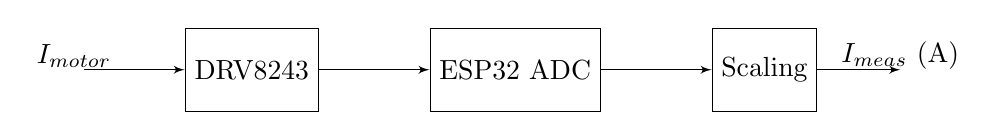
\begin{tikzpicture}
    \sbEntree{E}
    \sbBloc[4]{drv}{DRV8243}{E}
    \sbBloc[4]{adc}{ESP32 ADC}{drv}
    \sbBloc[4]{scale}{Scaling}{adc}
    \sbSortie[3]{S}{scale}

    \sbRelier{E}{drv}
    \sbRelier{drv}{adc}
    \sbRelier{adc}{scale}
    \sbRelier{scale}{S}

    \sbNomLien[0.5]{E}{$I_{motor}$}
    \sbNomLien[0.5]{S}{$I_{meas}$ (A)}
\end{tikzpicture}
\end{center}

\textbf{IPROPI Characteristics:}
\begin{itemize}
    \item Output: Analog voltage proportional to motor current
    \item Gain: \SI{1100}{\micro\ampere\per\ampere} (typical)
    \item With \SI{1}{\kilo\ohm} sense resistor: \SI{1.1}{\milli\volt\per\ampere}
    \item ESP32 ADC: 12-bit, \SI{0}{\volt} to \SI{3.3}{\volt} range
\end{itemize}

\begin{equation}
I_{motor} = \frac{V_{ADC}}{R_{sense} \cdot A_{IPROPI}} = \frac{V_{ADC}}{1000 \cdot 1100 \times 10^{-6}}
\end{equation}

% ============================================================================
% CHAPTER 4: SUPERVISORY SAFETY SYSTEM
% ============================================================================
\newpage
\section{Supervisory Safety System}

\subsection{Multi-Level Safety Architecture}

The STAR robot implements a \textbf{supervisory control layer} that can override the PID controllers for safety:

\begin{center}
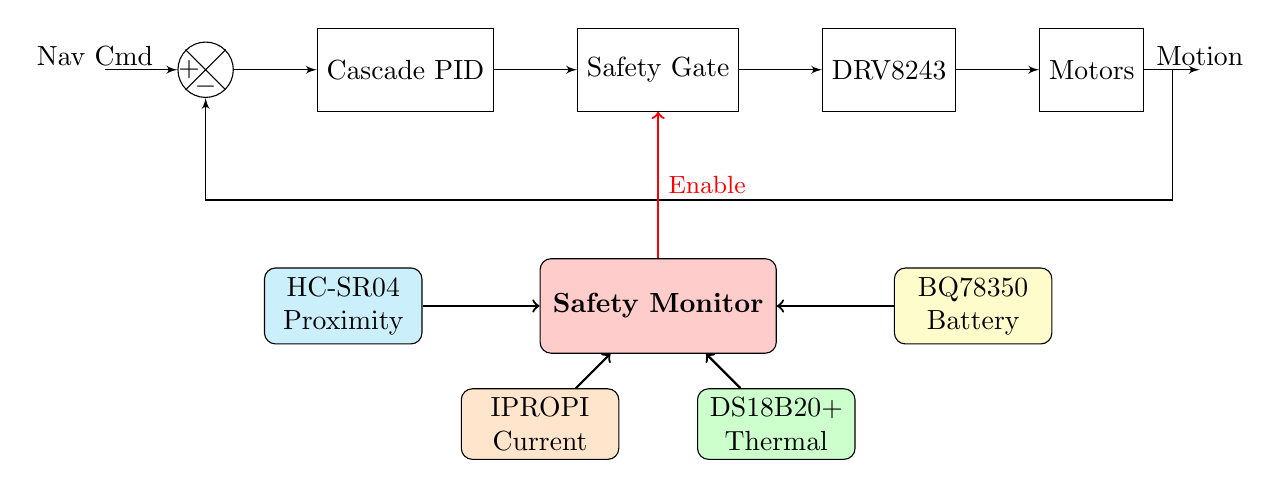
\begin{tikzpicture}
    % Main PID control path
    \sbEntree{E}
    \sbComp{sum}{E}
    \sbBloc[3]{pid}{Cascade PID}{sum}
    \sbBloc[3]{gate}{Safety Gate}{pid}
    \sbBloc[3]{drv}{DRV8243}{gate}
    \sbBloc[3]{motors}{Motors}{drv}
    \sbSortie[2]{S}{motors}

    % Main connections
    \sbRelier{E}{sum}
    \sbRelier{sum}{pid}
    \sbRelier{pid}{gate}
    \sbRelier{gate}{drv}
    \sbRelier{drv}{motors}
    \sbRelier{motors}{S}
    \sbRenvoi{motors-S}{sum}{}
    \sbNomLien[0.5]{E}{Nav Cmd}
    \sbNomLien[0.5]{S}{Motion}

    % Safety system block (below)
    \node[draw, fill=red!20, rounded corners, minimum width=3cm, minimum height=1.2cm, align=center]
        (safety) at ([yshift=-3cm]gate) {\textbf{Safety Monitor}};

    % Safety inputs
    \node[draw, fill=cyan!20, rounded corners, minimum width=2cm, align=center]
        (prox) at ([xshift=-4cm]safety) {HC-SR04\\Proximity};
    \node[draw, fill=orange!20, rounded corners, minimum width=2cm, align=center]
        (curr) at ([xshift=-1.5cm, yshift=-1.5cm]safety) {IPROPI\\Current};
    \node[draw, fill=green!20, rounded corners, minimum width=2cm, align=center]
        (temp) at ([xshift=1.5cm, yshift=-1.5cm]safety) {DS18B20+\\Thermal};
    \node[draw, fill=yellow!20, rounded corners, minimum width=2cm, align=center]
        (batt) at ([xshift=4cm]safety) {BQ78350\\Battery};

    % Safety connections
    \draw[->, thick, red] (safety) -- (gate) node[midway, right] {\small Enable};
    \draw[->, thick] (prox) -- (safety);
    \draw[->, thick] (curr) -- (safety);
    \draw[->, thick] (temp) -- (safety);
    \draw[->, thick] (batt) -- (safety);
\end{tikzpicture}
\end{center}

\subsection{Safety Conditions}

The Safety Gate implements the following conditions:

\begin{table}[H]
\centering
\begin{tabular}{@{}llll@{}}
\toprule
\textbf{Condition} & \textbf{Threshold} & \textbf{Action} & \textbf{Recovery} \\
\midrule
Proximity & $d < \SI{10}{\centi\meter}$ & Stop motors & $d > \SI{15}{\centi\meter}$ \\
Overcurrent & $I > \SI{8}{\ampere}$ & Reduce PWM & $I < \SI{6}{\ampere}$ \\
Thermal & $T > \SI{60}{\celsius}$ & Reduce power & $T < \SI{50}{\celsius}$ \\
Low Battery & $V < \SI{9.6}{\volt}$ & Safe shutdown & Manual reset \\
Stall Detect & $I > \SI{5}{\ampere}$, $\omega = 0$ & Stop motor & Manual reset \\
\bottomrule
\end{tabular}
\caption{Safety conditions with hysteresis thresholds}
\end{table}

\begin{safetynote}
All safety thresholds include \textbf{hysteresis} to prevent oscillation. For example, proximity detection turns off at 10cm but requires 15cm clearance to resume---this 5cm gap prevents flickering when objects are near the threshold.
\end{safetynote}

\subsection{State Machine}

The safety system operates as a state machine:

\begin{center}
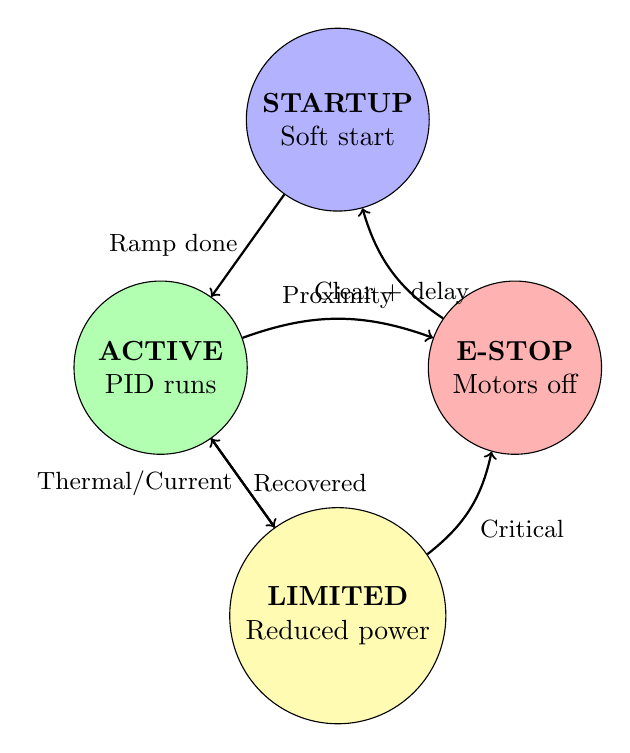
\begin{tikzpicture}[scale=0.9]
    % States
    \node[draw, circle, fill=green!30, minimum size=2.2cm, align=center] (active) at (0,0) {\textbf{ACTIVE}\\PID runs};
    \node[draw, circle, fill=red!30, minimum size=2.2cm, align=center] (estop) at (5,0) {\textbf{E-STOP}\\Motors off};
    \node[draw, circle, fill=yellow!30, minimum size=2.2cm, align=center] (limited) at (2.5,-3.5) {\textbf{LIMITED}\\Reduced power};
    \node[draw, circle, fill=blue!30, minimum size=2.2cm, align=center] (startup) at (2.5,3.5) {\textbf{STARTUP}\\Soft start};

    % Transitions
    \draw[->, thick] (active) to[bend left=20] node[above] {\small Proximity} (estop);
    \draw[->, thick] (estop) to[bend left=20] node[below] {\small Clear + delay} (startup);
    \draw[->, thick] (startup) -- (active) node[midway, left] {\small Ramp done};
    \draw[->, thick] (active) -- (limited) node[midway, left] {\small Thermal/Current};
    \draw[->, thick] (limited) -- (active) node[midway, right] {\small Recovered};
    \draw[->, thick] (limited) to[bend right=20] node[below right] {\small Critical} (estop);
\end{tikzpicture}
\end{center}

\subsection{Soft Start Implementation}

When transitioning from E-STOP to ACTIVE, we use a \textbf{soft start} ramp:

\begin{equation}
PWM(t) = PWM_{target} \cdot \left(3\left(\frac{t}{T_{ramp}}\right)^2 - 2\left(\frac{t}{T_{ramp}}\right)^3\right)
\end{equation}

This ``smoothstep'' function provides:
\begin{itemize}
    \item Zero velocity at start and end of ramp
    \item Smooth acceleration (no jerks)
    \item $T_{ramp} = \SI{1}{\second}$ default duration
\end{itemize}

\begin{whymatters}
Soft start prevents current spikes that could trip the overcurrent protection immediately after resuming. It also resets the PID integrators to prevent ``windup'' from the stopped period.
\end{whymatters}

% ============================================================================
% CHAPTER 5: SLAM AND NAVIGATION
% ============================================================================
\newpage
\section{SLAM and Navigation Layer}

\subsection{Hector-SLAM Overview}

The Raspberry Pi 5 runs \textbf{Hector-SLAM} for simultaneous localization and mapping:

\begin{center}
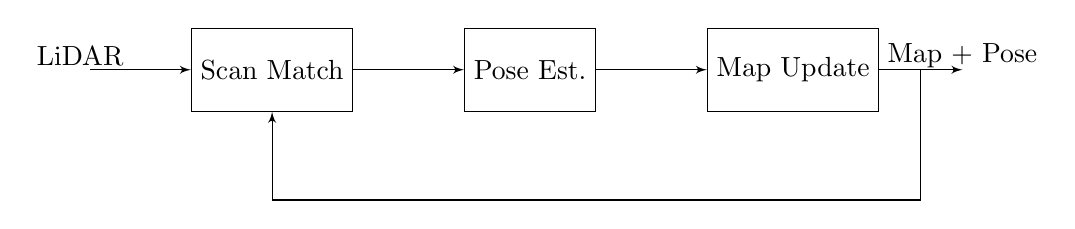
\begin{tikzpicture}
    \sbEntree{E}
    \sbBloc[4]{scan}{Scan Match}{E}
    \sbBloc[4]{pose}{Pose Est.}{scan}
    \sbBloc[4]{map}{Map Update}{pose}
    \sbSortie[3]{S}{map}

    \sbRelier{E}{scan}
    \sbRelier{scan}{pose}
    \sbRelier{pose}{map}
    \sbRelier{map}{S}

    \sbNomLien[0.5]{E}{LiDAR}
    \sbNomLien[0.5]{S}{Map + Pose}

    % Feedback
    \sbRenvoi{map-S}{scan}{}
\end{tikzpicture}
\end{center}

\textbf{Hector-SLAM Advantages:}
\begin{itemize}
    \item No odometry required (uses scan-matching only)
    \item Works well with high-frequency LiDAR (15Hz RPLiDAR C1)
    \item Real-time capable on RPi5
\end{itemize}

\subsection{Nav2 Path Planning}

ROS2 Nav2 provides the navigation stack:

\begin{center}
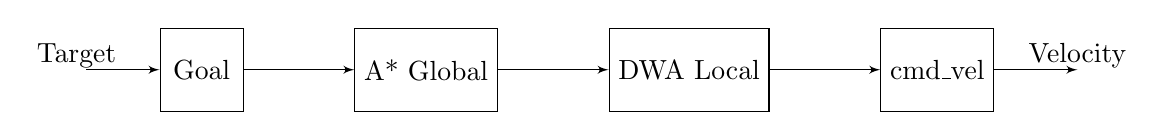
\begin{tikzpicture}
    \sbEntree{E}
    \sbBloc[3]{goal}{Goal}{E}
    \sbBloc[4]{global}{A* Global}{goal}
    \sbBloc[4]{local}{DWA Local}{global}
    \sbBloc[4]{cmd}{cmd\_vel}{local}
    \sbSortie[3]{S}{cmd}

    \sbRelier{E}{goal}
    \sbRelier{goal}{global}
    \sbRelier{global}{local}
    \sbRelier{local}{cmd}
    \sbRelier{cmd}{S}

    \sbNomLien[0.5]{E}{Target}
    \sbNomLien[0.5]{S}{Velocity}
\end{tikzpicture}
\end{center}

\textbf{Planning Layers:}
\begin{enumerate}
    \item \textbf{Global Planner (A*):} Finds optimal path on occupancy grid (1 Hz)
    \item \textbf{Local Planner (DWA):} Dynamic Window Approach for obstacle avoidance (10 Hz)
    \item \textbf{Velocity Smoother:} Ensures commands respect acceleration limits
\end{enumerate}

\subsection{SPI Communication Protocol}

The RPi5 sends velocity commands to ESP32 via SPI:

\begin{table}[H]
\centering
\begin{tabular}{@{}llll@{}}
\toprule
\textbf{Byte} & \textbf{Field} & \textbf{Type} & \textbf{Description} \\
\midrule
0 & Header & uint8 & 0xAA (start byte) \\
1-2 & Linear X & int16 & Linear velocity (mm/s) \\
3-4 & Linear Y & int16 & Lateral velocity (mm/s) \\
5-6 & Angular Z & int16 & Angular velocity (mrad/s) \\
7 & Checksum & uint8 & XOR of bytes 1-6 \\
\bottomrule
\end{tabular}
\caption{SPI command packet structure (8 bytes)}
\end{table}

\begin{ournumbers}
\textbf{Communication Parameters:}
\begin{itemize}[noitemsep]
    \item SPI Clock: \SI{1}{\mega\hertz}
    \item Mode: SPI Mode 0 (CPOL=0, CPHA=0)
    \item Command Rate: \SI{50}{\hertz} (matches control loop)
    \item Timeout: \SI{100}{\milli\second} (triggers E-STOP if exceeded)
\end{itemize}
\end{ournumbers}

% ============================================================================
% CHAPTER 6: STABILITY ANALYSIS
% ============================================================================
\newpage
\section{Stability Analysis}

\subsection{Loop Stability Requirements}

For cascaded control, each loop must be stable independently:

\begin{keypoint}
\textbf{Stability Rule for Cascaded Loops:}
\begin{enumerate}
    \item Inner loops must be faster than outer loops (bandwidth separation)
    \item Each loop must have positive gain and phase margins
    \item Typically: $\omega_{inner} > 5 \times \omega_{outer}$
\end{enumerate}
\end{keypoint}

\subsection{Bode Plot Analysis}

For the velocity loop with plant $G_v(s) = \frac{K_m}{(\tau_m s + 1)}$:

\begin{equation}
G_v(s) = \frac{10}{0.1s + 1}
\end{equation}

With PI controller $C_v(s) = K_p + \frac{K_i}{s} = 2.0 + \frac{0.5}{s}$:

Open-loop transfer function:
\begin{equation}
L_v(s) = C_v(s) \cdot G_v(s) = \frac{(2.0s + 0.5) \cdot 10}{s(0.1s + 1)}
\end{equation}

\subsection{Closed-Loop Poles}

The closed-loop transfer function:
\begin{equation}
T(s) = \frac{L(s)}{1 + L(s)}
\end{equation}

For stability, all poles must have negative real parts (left half-plane).

\begin{ournumbers}
\textbf{Expected Stability Margins:}
\begin{itemize}[noitemsep]
    \item Gain Margin: $>$ \SI{10}{\decibel} (target)
    \item Phase Margin: $>$ \SI{45}{\degree} (target)
    \item Crossover Frequency: \SI{10}{\radian\per\second} (velocity loop)
\end{itemize}
\end{ournumbers}

\subsection{Robustness Considerations}

The system must remain stable under:
\begin{itemize}
    \item Parameter variations (motor wear, temperature)
    \item Load disturbances (terrain changes)
    \item Sensor noise (ADC quantization, EMI)
    \item Communication delays (SPI latency)
\end{itemize}

\begin{whymatters}
We design for ``robust stability''---the system should work even when parameters change by $\pm$20\% from nominal. This is why we target generous stability margins rather than optimal performance.
\end{whymatters}

% ============================================================================
% CHAPTER 7: DISCRETE IMPLEMENTATION
% ============================================================================
\newpage
\section{Discrete-Time Implementation}

\subsection{Sampling Considerations}

The ESP32 runs the control loop at \SI{50}{\hertz} ($T_s = \SI{20}{\milli\second}$):

\begin{equation}
f_s = \SI{50}{\hertz}, \quad T_s = \SI{20}{\milli\second}
\end{equation}

\textbf{Nyquist Criterion:}
\begin{equation}
f_s > 2 \cdot f_{bandwidth}
\end{equation}

With velocity loop bandwidth of approximately \SI{10}{\radian\per\second} (\SI{1.6}{\hertz}):
\begin{equation}
\SI{50}{\hertz} > 2 \times \SI{1.6}{\hertz} = \SI{3.2}{\hertz} \quad \checkmark
\end{equation}

We have approximately 15x oversampling, which is excellent.

\subsection{Discrete PID Implementation}

Using Tustin (bilinear) transformation:

\begin{align}
P[n] &= K_p \cdot e[n] \\
I[n] &= I[n-1] + K_i \cdot T_s \cdot \frac{e[n] + e[n-1]}{2} \\
D[n] &= \alpha \cdot K_d \cdot \frac{e[n] - e[n-1]}{T_s} + (1-\alpha) \cdot D[n-1] \\
u[n] &= P[n] + I[n] + D[n]
\end{align}

Where $\alpha = 0.1$ is the derivative filter coefficient.

\subsection{Anti-Windup Implementation}

To prevent integral windup during saturation:

\begin{verbatim}
// Conditional integration
if (output_saturated) {
    // Don't accumulate integral when output is limited
    integral_term = integral_term;  // Hold
} else {
    integral_term += Ki * Ts * (error + prev_error) / 2.0;
}

// Clamp integral term
integral_term = constrain(integral_term, -I_MAX, I_MAX);
\end{verbatim}

\subsection{Code Structure}

\begin{verbatim}
void control_loop_50Hz() {
    // 1. Read sensors
    float pos = read_encoders();
    float vel = read_bno055_velocity();
    float current = read_ipropi();

    // 2. Check safety conditions
    if (check_safety_conditions() != SAFE) {
        enter_estop();
        return;
    }

    // 3. Position loop (outer)
    float vel_setpoint = position_pid(pos_setpoint, pos);

    // 4. Velocity loop (middle)
    float cur_setpoint = velocity_pid(vel_setpoint, vel);

    // 5. Current loop (inner)
    float pwm = current_pid(cur_setpoint, current);

    // 6. Apply output
    set_motor_pwm(pwm);
}
\end{verbatim}

% ============================================================================
% CHAPTER 8: HARDWARE SPECIFICATIONS
% ============================================================================
\newpage
\section{Hardware Specifications}

\subsection{Motor System}

\begin{table}[H]
\centering
\begin{tabular}{@{}ll@{}}
\toprule
\textbf{Parameter} & \textbf{Value} \\
\midrule
Motor Type & DC Brushed with Encoder \\
Voltage & \SI{12}{\volt} nominal \\
Stall Current & \SI{3}{\ampere} \\
No-Load Speed & \SI{500}{RPM} \\
Encoder Resolution & 500 PPR (2000 CPR quadrature) \\
Quantity & 4 (differential drive, 4WD) \\
\bottomrule
\end{tabular}
\caption{Motor specifications}
\end{table}

\subsection{Motor Driver (DRV8243-Q1)}

\begin{table}[H]
\centering
\begin{tabular}{@{}ll@{}}
\toprule
\textbf{Parameter} & \textbf{Value} \\
\midrule
Configuration & Dual H-Bridge \\
Continuous Current & \SI{12}{\ampere} per channel \\
Peak Current & \SI{24}{\ampere} \\
PWM Frequency & \SI{20}{\kilo\hertz} \\
Current Sense & IPROPI analog output \\
Protection & Overcurrent, thermal shutdown \\
Quantity & 2 (one per motor pair) \\
\bottomrule
\end{tabular}
\caption{DRV8243-Q1 specifications}
\end{table}

\subsection{Power System}

\begin{table}[H]
\centering
\begin{tabular}{@{}lll@{}}
\toprule
\textbf{Rail} & \textbf{Voltage} & \textbf{Current Capacity} \\
\midrule
Battery & \SI{11.1}{\volt} (3S LiPo) & \SI{5000}{\milli\ampere\hour} \\
Motor Power & \SI{12}{\volt} (regulated) & \SI{24}{\ampere} max \\
Logic 5V & \SI{5}{\volt} & \SI{3}{\ampere} \\
Logic 3.3V & \SI{3.3}{\volt} & \SI{500}{\milli\ampere} \\
\bottomrule
\end{tabular}
\caption{Power distribution}
\end{table}

\subsection{Processor Specifications}

\begin{table}[H]
\centering
\begin{tabular}{@{}lll@{}}
\toprule
\textbf{Parameter} & \textbf{Raspberry Pi 5} & \textbf{ESP32} \\
\midrule
CPU & Cortex-A76 Quad @ \SI{2.4}{\giga\hertz} & Xtensa Dual @ \SI{240}{\mega\hertz} \\
RAM & \SI{4}{\giga\byte} & \SI{520}{\kilo\byte} \\
Role & SLAM, Navigation & Motor Control \\
OS & Ubuntu 22.04 + ROS2 & FreeRTOS \\
Control Rate & \SI{10}{\hertz} (Nav2) & \SI{50}{\hertz} (PID) \\
\bottomrule
\end{tabular}
\caption{Processing units comparison}
\end{table}

\begin{ournumbers}
\textbf{Total System Budget:}
\begin{itemize}[noitemsep]
    \item Raspberry Pi 5 (4GB): \$60
    \item ESP32 DevKit: \$10
    \item DRV8243-Q1 (x2): \$15
    \item Motors with encoders (x4): \$80
    \item RPLiDAR C1: \$100
    \item BNO055 IMU: \$30
    \item Sensors and passives: \$25
    \item Power system: \$50
    \item Chassis and hardware: \$80
    \item \textbf{Total:} Approximately \$450
\end{itemize}
\end{ournumbers}

% ============================================================================
% APPENDIX A: GLOSSARY
% ============================================================================
\newpage
\section*{Appendix A: Glossary}
\addcontentsline{toc}{section}{Appendix A: Glossary}

\begin{table}[H]
\begin{tabular}{@{}p{3.5cm}p{10.5cm}@{}}
\toprule
\textbf{Term} & \textbf{Definition} \\
\midrule
\textbf{Cascaded Control} & Multiple nested control loops where the output of an outer loop is the setpoint for an inner loop \\
\textbf{DWA} & Dynamic Window Approach---local path planning algorithm \\
\textbf{Hector-SLAM} & Scan-matching SLAM algorithm that doesn't require odometry \\
\textbf{IPROPI} & Current sense output pin on DRV8243-Q1 motor driver \\
\textbf{Nav2} & ROS2 Navigation Stack for autonomous mobile robots \\
\textbf{Nyquist Rate} & Minimum sampling rate (2x bandwidth) to avoid aliasing \\
\textbf{SLAM} & Simultaneous Localization and Mapping \\
\textbf{Soft Start} & Gradual ramp-up of motor power to prevent current spikes \\
\textbf{Supervisory Control} & Higher-level control layer that can override lower loops \\
\textbf{Tustin Transform} & Bilinear transformation for converting continuous to discrete \\
\bottomrule
\end{tabular}
\end{table}

% ============================================================================
% APPENDIX B: BLOCK DIAGRAM REFERENCE
% ============================================================================
\newpage
\section*{Appendix B: Schemabloc Quick Reference}
\addcontentsline{toc}{section}{Appendix B: Schemabloc Reference}

\begin{table}[H]
\centering
\begin{tabular}{@{}ll@{}}
\toprule
\textbf{Command} & \textbf{Description} \\
\midrule
\verb|\sbEntree{name}| & Create input node \\
\verb|\sbSortie[dist]{name}{ref}| & Create output node \\
\verb|\sbBloc[dist]{name}{label}{ref}| & Create processing block \\
\verb|\sbComp{name}{ref}| & Create comparator/summer \\
\verb|\sbRelier[label]{from}{to}| & Connect nodes \\
\verb|\sbRenvoi{from}{to}{label}| & Create feedback path \\
\verb|\sbNomLien[pos]{ref}{text}| & Label a connection \\
\verb|\sbBlocr{name}{label}{ref}| & Feedback block (reversed) \\
\verb|\sbRelieryx{from}{to}| & Vertical-then-horizontal path \\
\verb|\sbRelierxy{from}{to}| & Horizontal-then-vertical path \\
\bottomrule
\end{tabular}
\caption{Essential schemabloc commands}
\end{table}

\textbf{Basic Closed-Loop Example:}
\begin{verbatim}
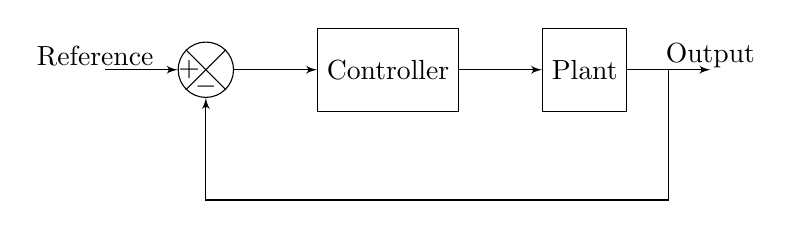
\begin{tikzpicture}
    \sbEntree{E}
    \sbComp{sum}{E}
    \sbBloc[3]{ctrl}{Controller}{sum}
    \sbBloc[3]{plant}{Plant}{ctrl}
    \sbSortie[3]{S}{plant}
    \sbRelier{E}{sum}
    \sbRelier{sum}{ctrl}
    \sbRelier{ctrl}{plant}
    \sbRelier{plant}{S}
    \sbRenvoi{plant-S}{sum}{}
    \sbNomLien[0.5]{E}{Reference}
    \sbNomLien[0.5]{S}{Output}
\end{tikzpicture}
\end{verbatim}

% ============================================================================
% APPENDIX C: QUICK REFERENCE
% ============================================================================
\newpage
\section*{Appendix C: Demo Quick Reference}
\addcontentsline{toc}{section}{Appendix C: Quick Reference}

\begin{table}[H]
\centering
\begin{tabular}{@{}ll@{}}
\toprule
\textbf{Parameter} & \textbf{Value} \\
\midrule
\multicolumn{2}{@{}l@{}}{\textbf{Control Loop Rates}} \\
Position Loop & \SI{10}{\hertz} (from Nav2) \\
Velocity Loop & \SI{50}{\hertz} \\
Current Loop & \SI{50}{\hertz} \\
Safety Monitor & \SI{50}{\hertz} \\
\midrule
\multicolumn{2}{@{}l@{}}{\textbf{Safety Thresholds}} \\
Proximity Stop & $< \SI{10}{\centi\meter}$ \\
Proximity Resume & $> \SI{15}{\centi\meter}$ \\
Overcurrent Limit & $> \SI{8}{\ampere}$ \\
Thermal Limit & $> \SI{60}{\celsius}$ \\
Low Battery & $< \SI{9.6}{\volt}$ \\
\midrule
\multicolumn{2}{@{}l@{}}{\textbf{Communication}} \\
SPI Clock & \SI{1}{\mega\hertz} \\
Command Packet & 8 bytes \\
Timeout & \SI{100}{\milli\second} \\
\midrule
\multicolumn{2}{@{}l@{}}{\textbf{PID Gains (Initial)}} \\
Position: $K_p, K_i$ & 1.0, 0.1 \\
Velocity: $K_p, K_i, K_d$ & 2.0, 0.5, 0.05 \\
Current: $K_p, K_i$ & 5.0, 100 \\
\bottomrule
\end{tabular}
\caption{Quick reference values for demo}
\end{table}

\subsection*{Common Demo Questions}

\textbf{Q: Why two processors?}

A: The RPi5 handles computationally expensive SLAM (scan matching, map updates) while the ESP32 runs time-critical motor control at a guaranteed 50Hz. This separation ensures smooth motion even during heavy mapping computation.

\vspace{0.3cm}

\textbf{Q: Why cascaded PID instead of single loop?}

A: Cascaded control lets us protect the motors (current limit), maintain smooth speed (velocity loop), and reach positions accurately (position loop)---all independently tunable.

\vspace{0.3cm}

\textbf{Q: What happens if communication fails?}

A: The ESP32 has a 100ms timeout. If no SPI commands arrive, it triggers E-STOP and stops all motors. The robot will remain stopped until communication is restored and manually reset.

\vspace{0.3cm}

\textbf{Q: How does temperature affect the ultrasonic sensor?}

A: Sound speed varies with temperature (\SI{0.6}{\meter\per\second} per degree C). Without compensation, measurements could be off by several millimeters. The DS18B20+ provides real-time temperature for correction.

\end{document}
